\subsection{Закон великих чисел (ЗВЧ).}

Маємо $\xi_1, \xi_2, ...$, тоді:
$$
\underbrace{\frac{\xi_1 + \xi_2 + ... + \xi_n}{n}}_{\text{вибіркове середнє}} \xrightarrow[n \to \i]{} \mathbb{E}\xi
$$
\begin{boxteo}(ЗВЧ для незалежних, однаково розподілених величин)\\
  $\xi_1, \xi_2, ..., \xi_n$ - незалежні, однаково розподілені випадкові величини.\\
  Нехай $\exists\mathbb{E}\xi_i = a$.
  \textbf{Тоді}:
  $$
  \frac{\xi_1 + ... + \xi_n}{n} \xrightarrow[n \to \i]{\mathbb{P}} a
\qquad
  \left( \mathbb{P} \left\lbrace \frac{\xi_1 + ... + \xi_n}{n}  > \varepsilon  \right\rbrace \xrightarrow[n \to \i]{} 0 \right)
  $$
\end{boxteo}
\begin{proof} ( за додаткової умови існування дисперсії $\exists\mathbb{D}\xi_i$, що , але з послабленим припущенням про некорельованість замість незалежності.)
$$
\overline{\xi} = \frac{\xi_1 + ... + \xi_n}{n} : \begin{gathered}
 \mathbb{E} \overline{\xi}_n= \mathbb{E}  \frac{\xi_1 + ... + \xi_n}{n}  = \frac{ \mathbb{E}\xi_1 + ... + \mathbb{E}\xi_n}{n}  = \frac{na}{a} = a \\
 \mathbb{D} \overline{\xi}_n = \mathbb{D} \frac{\xi_1 + ... + \xi_n}{n} = \frac{\mathbb{D}\xi_1 + ... + \mathbb{D}\xi_n}{n^2} =  \frac{n \mathbb{D} \xi}{ n^2} = \frac{\mathbb{D} \xi}{n}
\end{gathered}
$$
$$
\begin{dcases}
 \mathbb{E} \overline{\xi}_n = a \xrightarrow[n\to \i]{} a \\
 \mathbb{D} \overline{\xi}_n = \frac{\mathbb{D} \xi}{n} \xrightarrow[n\to \i]{} 0
 \end{dcases} \Longrightarrow \overline{\xi}_n \xrightarrow[n\to \i]{\mathbb{L}_2} a \Longrightarrow \overline{\xi}_n \xrightarrow[n\to \i]{\mathbb{P} } a
$$
\end{proof}

\begin{proof} (без припущення про існування $\mathbb{D} \xi$)\\
Введемо характеристичну функцію $ \char (t) = \mathbb{E} e^{it \xi}$. Тоді:
$$
    \chi_{\frac{\xi_1 + ... + \xi_n}{n}}(t) =  \mathbb{E} e ^{ \frac{it}{n} (\xi_1 + ... + \xi_n)  } = \chi_{\xi_1 + ... + \xi_n} \left( \frac{t}{n}  \right) = \underbrace{\char \left( \frac{t}{n}  \right)\cdot ... \cdot \char \left( \frac{t}{n}  \right)}_{n} = \char^n \left( \frac{t}{n}  \right)
$$
Розпишемо в ряд Тейлора:
$$
\char(h)  = \char(0) + \frac{\char'(0)}{1!} h + o(h) \quad h \to 0
$$
$$
\char(h)  =  \left| \frac{\char'(0)}{i}  = \mathbb{E}\xi \right|= 1 + ia\cdot h + o(h) \quad h \to 0
$$
$$
\char \left( \frac{t}{n} \right)   =  1 + \frac{iat}{n}  + o( \frac{1}{n} ) \quad n \to \i
$$
Отримали:
$$
\chi_{\overline{\xi}_n} (t) = \char^n \left( \frac{t}{n}  \right) = \left[ 1 + \frac{iat}{n}  + o  \left( \frac{1}{n} \right)\right]^n  \quad n \to \i
$$
$$
\ln{ \chi_{\overline{\xi}_n} (t) } = n \ln \left[ 1 + \frac{iat}{n}  + o  \left( \frac{1}{n} \right) \right] \sim n \left[ \frac{iat}{n} + o \left( \frac{1}{n}  \right)  \right] = iat + o(1) \xrightarrow[n\to \i]{} a
$$
$$
\chi_{\overline{\xi}_n} (t) \xrightarrow[ n \to \infty]{} e^{iat} = \mathbb{E} e^{iat}= \char (t) \quad \fbox{$\xRightarrow{\text{т. Леві}}$}
$$
$$
\fbox{$\Longrightarrow$} \overline{\xi}_n = \frac{\xi_1 + ... + \xi_n}{n} \xrightarrow[n\to\i]{d}a \Rightarrow \fbox{$\dfrac{\xi_1 + ... + \xi_n}{n} \xrightarrow[n\to\i]{\mathbb{P}} a$}
$$
% Missing data
\end{proof}
\begin{boxteo}(посилений ЗВЧ А.М.Колмогорова.)\\
$\xi_1, \xi_2, ..., \xi_n$ - незалежні, однаково розподілені випадкові величини.
$$
\text{Нехай } \exists\mathbb{E}\xi_i = a.\
\textbf{Тоді:}\  \frac{\xi_1 + ... + \xi_n}{n} \xrightarrow[n \to \i]{\textbf{м.н.}} a
$$
\end{boxteo}
\subsection{ЗВЧ для різнорозподілених випадкових величин.}
\subsubsection{Означення.}
\begin{boxteo}
$\xi_1, \xi_2, ..., \xi_n$ - незалежні випадкові величини.
Нехай $\begin{gathered}
 \exists\mathbb{E}\xi_i = a_i\\
 \exists \mathbb{D} \xi_i = \sigma^2_i
\end{gathered}$. \\ Додатково накладемо умову рівномірної обмеженості:  $\exists C > 0:  \sigma^2_i < C $.
$$
 \textbf{Тоді:} \ \frac{ \xi_1 + ... + \xi_n}{n} - \frac{a_1 + ... + a_n}{n} = \frac{(\xi_1 - a_1) + ... + (\xi_n - a_n)}{n}   \xrightarrow[n\to \i]{\mathbb{P}, \mathbb{L}_2} 0
$$
\end{boxteo}
\begin{proof}
 $$
 \begin{dcases}
   \mathbb{E} \left( \frac{(\xi_1 - a_1) + ... + (\xi_n - a_n)}{n}  \right)= \frac{\overbrace{\mathbb{E}(\xi_1 - a_1)}^{=0} + ... +\overbrace{\mathbb{E}(\xi_n - a_n)}^{=0}}{n} =  0  & \xrightarrow[n\to\i]{} 0\\
   \mathbb{D} \left(  \frac{(\xi_1 - a_1) + ... + (\xi_n - a_n)}{n} \right) =   \frac{\mathbb{D}(\xi_1 - a_1) + ... + \mathbb{D}(\xi_n - a_n)}{n^2} = \\
   = \frac{\mathbb{D} \xi_1 + ... + \mathbb{D}\xi_n}{n} - \frac{a_1 + ... + a_n}{n^2} = \frac{\sigma_1 ^2 + ... + \sigma_n^2}{n^2} \leq \frac{C\cdot n}{n^2} = \frac{C}{n} &\xrightarrow[n\to\i]{} 0
 \end{dcases}
 $$
 З цього слідує: $ \frac{(\xi_1 - a_1) + ... + (\xi_n - a_n)}{n} \xrightarrow[n\to\i]{\mathbb{L}_2, \mathbb{P}}
 0 $
\end{proof}

\subsubsection{ЗВЧ для схеми Бернуллі.}
Успіх: $p$. Невдача: $q = 1 - p$. \\
Введемо величину $\xi_i = \index{} \left\lbrace \text{на i-тому випробуванні відбувся успіх} \right\rbrace$
$$
\begin{gathered}
  \begin{gathered}
   \xi_i \\
   \mathbb{P}
  \end{gathered}
  \
  \begin{gathered}
   0\\
   q
  \end{gathered}
  \
  \begin{gathered}
   1 \\
   p
  \end{gathered} \quad \mathbb{E} \xi_i = p
\end{gathered}
$$
За ЗВЧ Колмогорова:
$$
\frac{\xi_1 + ... + \xi_n}{n} \xrightarrow[n \to \i]{\mathbb{L}_2, \mathbb{P}, \text{м.н}}  \mathbb{E} \xi_i = p
$$
$\frac{\xi_1 + ... + \xi_n}{n} $ - відносна частота успіхів $ = \nu_n \Longrightarrow $ \fbox{ $\nu_n \xrightarrow[n \to \i]{\mathbb{L}_2, \text{м.н}} p $}


\subsubsection{Методи Монте-Карло.}
\textbf{Приклад.} Методи Монте-Карло дозволяють чисельно розв'язувати нестохастичні (детерміновані) задачі задопомогою стохастичних методів.\\
Шукаємо приблизне значення
$ \displaystyle \int\limits_{b}^{a}{f(x)dx }$ при  $ M \geq  f(x) \geq 0 $ -  обмежена на $[a,b]$ .\\
\begin{center}
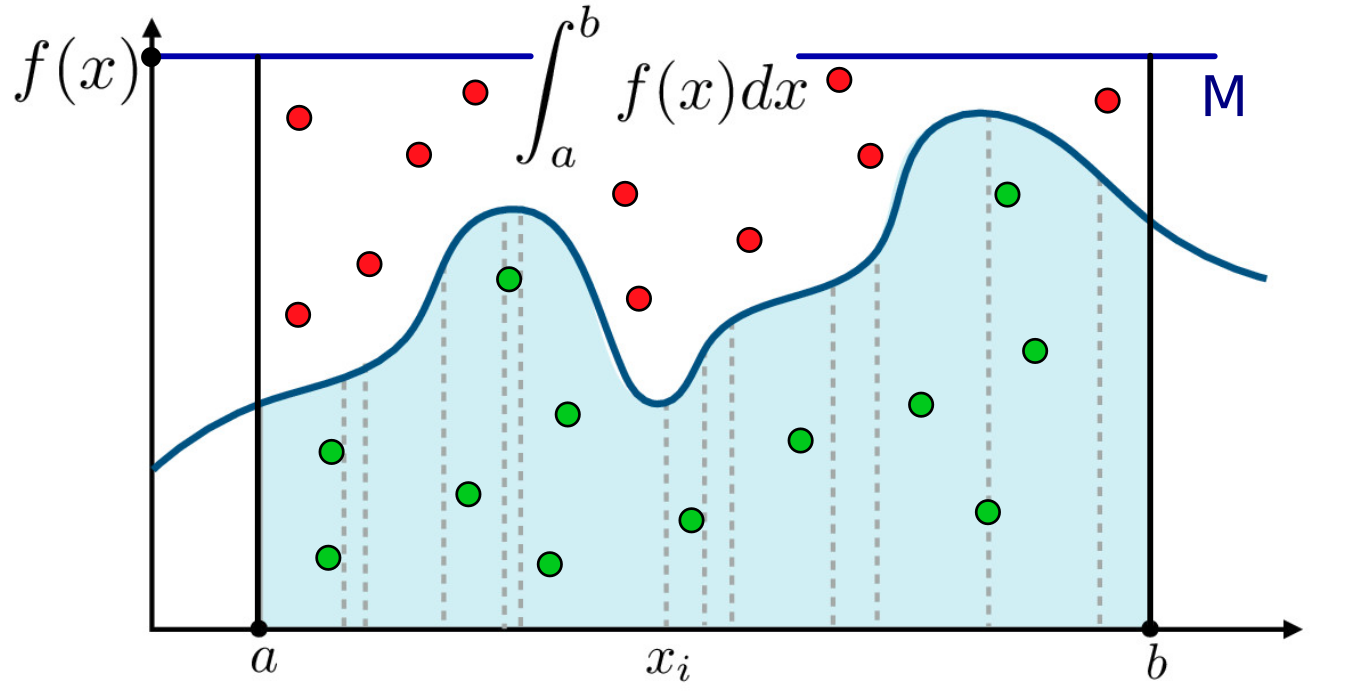
\includegraphics[scale=0.33]{assets/lectures_part_4-fdb5d503.png}
Вибираємо незалежні: $\xi_n \sim U(a,b)$.
\end{center}
$f(\xi_1), ... f(\xi_n) $ - незалежні, однаково розподілені з математичним сподіванням:
$$
\mathbb{E} f(\xi_i) =  \int\limits_{b}^{ a}{ f(x) \cdot \frac{1}{b-a}dx } = \frac{1}{b-a}  \int\limits_{b}^{a}{f(x)dx}
$$
Застосуємо закон великих чисел:
$$
\frac{f(\xi_1) + ... + f(\xi_n)}{n} \xrightarrow[n \to \i]{\text{м.н.}}  \mathbb{E} f(\xi)
$$
Якщо взяти $ n >> 1$:
$$
\frac{f(\xi_1) + ... + f(\xi_n)}{n} \approx \frac{1}{b-a}  \int\limits_{b}^{a}{f(x)dx}
$$
Інакше:
$$  \int\limits_{b}^{a}{f(x)dx} \approx \left( b-a \right)\cdot \frac{f(\xi_1) + ... + f(\xi_n)}{n}$$
\begin{example}(Другий спосіб) Розглядаємо прямокутник $\Pi = (a,b) \times M$.\\
Випадкові вектори $\begin{bmatrix}
 \xi_1 \\
 \eta_1
\end{bmatrix}, \cdots , \begin{bmatrix}
 \xi_n\\
 \eta_n
\end{bmatrix} $ - точки всередині прямокутника $ \Pi$.\\
Схема Бернуллі: $n$ випробувань. Успіх: потрапляння точки під графік $f(x)$.
$$
p = \mathbb{P} \left\lbrace \text{успіх} \right\rbrace = \frac{S_{\text{під графіком}}}{S_{\Pi}} =
\frac{ \int\limits_{b}^{a}{f(x)dx}}{M(b-a)}
$$
Частота влучання під графік: $\nu_n \xrightarrow[n \to \i]{\text{м.н}} p = \frac{ \int\limits_{b}^{a}{f(x)dx}}{M(b-a)}  $.\\
Якщо $ n >> 1$, то $ \int\limits_{b}^{a}{f(x)dx} \approx M(b-a)\nu_n = M(b-a)\cdot \frac{\text{к-сть точок під графіком}}{n} $.

\end{example}
